\chapter{QUADRO METODOLÓGICO}

	\par Nesse capítulo serão apresentados os métodos adotados para se realizar a
pesquisa, tais como tipo de pesquisa, contexto, procedimentos, entre outros.

\section{Tipo de pesquisa}
	
	\par Uma pesquisa é o ato de buscar e procurar pela resposta de algo.
\citeonline[p. 15]{markoni2002} definem pesquisa como “uma indagação minuciosa
ou exame crítico e exaustivo na procura de fatos e princípios”.

	\par Existem diversos tipos de pesquisa, no entanto percebeu-se que para o
propósito desta, a mais indicada foi a pesquisa aplicada, pois está se
desenvolvendo um projeto real que poderá ser utilizado por qualquer instituição
de ensino, mas que não mudará a forma com que as pessoas recebam suas
informações, apenas acrescenta mais uma forma de consultá-las.

	\par Segundo \citeonline[p. 15]{markoni2002}, uma pesquisa do tipo aplicada
“caracteriza-se por seu interesse prático, isto é, que os resultados sejam
aplicados ou utilizados, imediatamente, na solução de problemas que ocorrem na
realidade”.

	\par Dessa maneira, percebeu-se que a pesquisa enquadra-se no tipo de pesquisa
aplicada, pois com a execução da mesma resolve-se um problema específico, e para
isso está desenvolvendo-se um aplicativo para dispositivos móveis que facilitará aos
graduandos acessarem o sistema \textit{web} de uma universidade.

\section{Contexto de pesquisa}

	\par Essa pesquisa será benéfica a qualquer instituição educacional que possua
um portal \textit{online}, pois facilitará o acesso dos discentes às suas
informações escolares.

	\par Está em fase de criação um aplicativo para dispositivos móveis, porém
inicialmente apenas para a plataforma \textit{Android}, o qual notifica os
usuários quando há alguma mudança, como por exemplo, ao ser lançada uma nota.
	
	\par O aluno consegue acessar o aplicativo com o mesmo \textit{login} do
sistema \textit{web}. O utilitário acessa o \textit{webservice} que é
responsável por buscar as informações no banco de dados e apresentá-las no
dispositivo.
	
\section{Instrumentos}

	\par Pode-se dizer que um questionário é uma forma de coletar informações
através de algumas perguntas feitas a um público específico. Segundo
\citeonline{gunther2003}, questionário pode ser definido como um conjunto
de perguntas que mede a opinião e interesse do respondente.
	
	\par Foi realizado um questionário simples, que esta apresentado na figura
\ref{fig:exemplo4}, contendo quatro perguntas e enviado para \textit{e-mails} de
alguns alunos da universidade. O foco desse questionário era saber o motivo pelo qual
os usuários mais acessavam o portal do aluno e se tinham alguma dificuldade em
encontrar o que procuravam. Obteve-se um total de treze respostas, no qual
pode-se perceber que a maioria dos entrevistados afirmam terem dificuldades
para encontrar o que precisam e que o sistema não avisa quando ocorre alguma
alteração. Sobre o motivo do acesso cem por cento respondeu que entram no
sistema web para consultar suas notas.

\begin{figure}[h!]
	\centerline{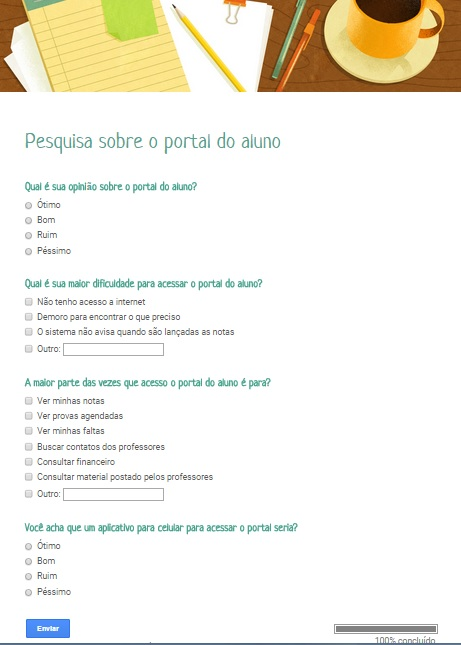
\includegraphics[scale=0.5]{./imagens/imagem4.png}}
	\caption[Quetionário Aplicado]{Quetionário Aplicado.
	 \textbf{Fonte:}Elaborado pelos autores.}
	\label{fig:exemplo4}
\end{figure}

\pagebreak

	\par Outra forma utilizada para realizar a pesquisa foram as reuniões, ou seja,
unir-se com uma ou mais pessoas em um local, físico ou remotamente para tratar
algum assunto específico. Para \citeonline{ferreira1999}, reunião é o ato
de encontro entre algumas pessoas em um determinado local, com finalidade de tratar
qualquer assunto.

	\par Durante a pesquisa, foram realizadas reuniões entre os participantes com o
objetivo de discutir o andamento das tarefas pela qual cada integrante ficou
responsável. Além disso entravam em discussão, nessas reuniões, o cumprimento
das metas propostas por cada participante e o estabelecimento de novas metas.
Foi utilizada nessa pesquisa, referências de livros, revistas, manuais e web
sites.


\section{Procedimentos}
	
	\par O primeiro procedimento realizado para chegar a pesquisa proposta, foi
planejar o \textit{software} através da linguagem UML, que necessitou a
instalação da ferramenta \textit{Astah} na sua versão 6.8.0.37.

	\par Como o planejamento é um passo importante, para o aplicativo Android,
fez-se necessários os diagramas de classe, de caso de uso principal e de
atividade.
	
	\par Para a contrução do \textit{software} proposto por essa pesquisa além do
levantamento de requisitos que é peculiar da contrução de qualquer
\textit{software}, 

	\begin{itemize}
	  \item Diagrama de casos de uso; 
	  \item Diagrama de sequência;
	  \item Diagrama de Entidade e Relacionamento (ou Modelo de Entidade e
	  Relacionamento )	
	\end{itemize}
	
	
	\par Para iniciar o desenvolvimento do aplicativo, primeiramente fez-se
necessária a instalação e configuração da plataforma \textit{Android Studio}
versão 1.1.0 e \textit{Android SDK}versão 24.0.2. Ao concluir essa tarefa,
deu-se o início ao aplicativo \textit{Android}.

	\par O primeiro passo foi a criação de uma \textit{activity main}, denominada
\texttt{MainActivity}, a qual será executada  quando a aplicação  for iniciada.
O tipo de \textit{activity} escolhida é chama-se \textit{Navigation Drawer
Layout}. Na figura \ref{fig:exemplo6} pode-se ver o método
\texttt{onNavigationDrawerItemSelected()}, que tem por finalidade mostrar as
opções de navegação e o que deverá acontecer quando uma delas for clicada. 
	
		\begin{figure}[h!]
			\centerline{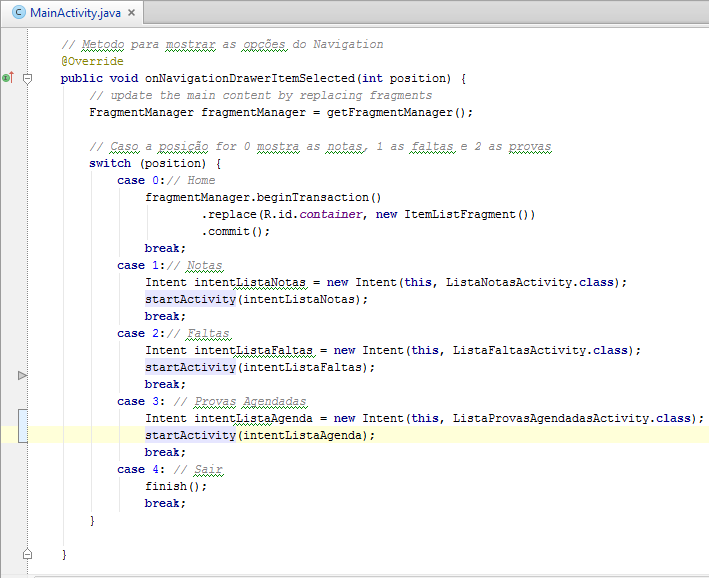
\includegraphics[scale=0.5]{./imagens/imagem6.png}}
			\caption[Implementação do
			método \texttt{onNavigationDrawerItemSelected()}]{Implementação do
			método \texttt{onNavigationDrawerItemSelected()}.
			 \textbf{Fonte:}Elaborado pelos autores.}
			\label{fig:exemplo6}
		\end{figure}
	
	\par Ao executa-la, funcionará como um menu, com as opções \textit{Home},
Notas, Faltas, Provas Agendadas e Sair. Essas opções ficam escondidas e só apareceram
quando clicado no canto superior esquerdo como mostra a figura
\ref{fig:exemplo7}.
		
		\begin{figure}[h!]
			\centerline{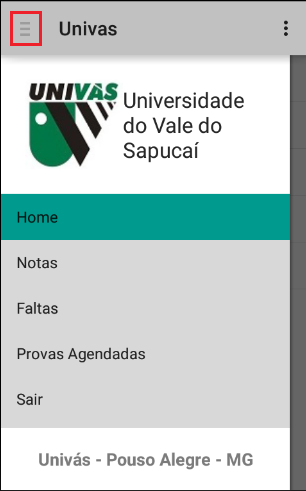
\includegraphics[scale=0.5]{./imagens/imagem7.png}}
			\caption[Representação Visual de
			\texttt{onNavigationDrawerItemSelected()}]{Representação Visual de
			\texttt{onNavigationDrawerItemSelected()}.
			 \textbf{Fonte:}Elaborado pelos autores.}
			\label{fig:exemplo7}
		\end{figure}
	
	\par Sempre que a aplicação é iniciada ou quando o usuário retorna para a
\textit{Home}, é apresentada uma lista com acesso a sites úteis. Para que essa
lista aparecesse foi utilizada uma \textit{activity} do tipo
\textit{Master/Deital Flow} que já traz consigo o \textit{widget} de
\textit{ListView}. Essa \textit{activity} mostrará as seguintes opções: Univás,
MEC, Fies, Prouni e Google Acadêmico. Ao clicar em um desses itens, será
chamada uma atividade que mostrará os detalhes do item escolhido, nesse caso na
\textit{activity} que detalhará o item foi utilizada um \textit{widget WebView}
que mostrará a página \textit{web} no espaço reservado. Dessa maneira, quando
for clicado na opção Univás será carregada o site da universidade no
aplicativo. Na figura \ref{fig:exemplo8}, é possível ver a tela  \textit{Home}
do aplicativo.
	
	\begin{figure}[h!]
			\centerline{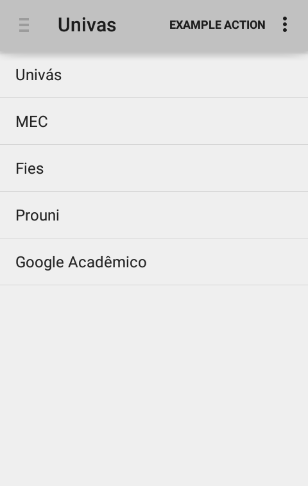
\includegraphics[scale=0.5]{./imagens/imagem8.png}}
			\caption[\textit{Activity Home} do aplicativo]{\textit{Activity Home} do aplicativo.
			 \textbf{Fonte:}Elaborado pelos autores.}
			\label{fig:exemplo8}
		\end{figure}
	
	\pagebreak	
	\par Logo após foram criadas três novas \textit{activities} do tipo
\textit{Blank Activity}, as quais listarão as matérias cursadas pelo aluno.
Nelas foram inseridas o \textit{widget ExpandableListView}, para que quando
clicado em um item listado, ele expandido mostre seus detalhes. Com isso quando
se escolhe o menu notas, será apresentada uma \textit{activity} que listará
todas as disciplinas cursadas e ao clicar em uma delas mostrará as notas
referente a ela. Na figura \ref{fig:exemplo9}, é possível ver uma
\textit{activity}, que lista algumas matérias e ao clicar em uma delas foi
possível ver as notas.
	
	\begin{figure}[h!]
			\centerline{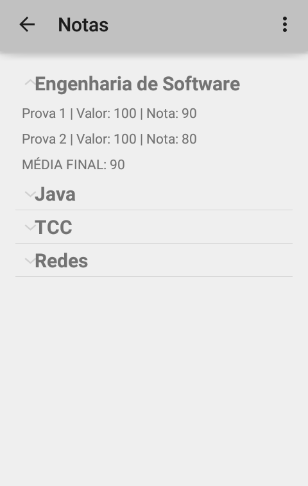
\includegraphics[scale=0.5]{./imagens/imagem9.png}}
			\caption[\textit{Activity} Notas]{\textit{Activity} Notas.
			 \textbf{Fonte:}Elaborado pelos autores.}
			\label{fig:exemplo9}
		\end{figure}
		
	\par Foi criada uma classe chamada \texttt{BuscaDados}, que tem por finalidade
receber os dados do \textit{webservice}, salvá-los no banco de dados local do
aplicativo e os entregar para as classes que implementam o \textiy{Adapter}
para listar as informações na tela do dispositivo.
	
	\par No arquivo \texttt{AndroidManifest.xml} foi necessário alterar a opção
\texttt{Android:icon}, que define qual será o ícone do aplicativo, por padrão
ele apresenta o mascote do \textit{Android}, no entanto foi definida uma imagem
do logo da universidade. Foi necessário também incluir uma tag de
\texttt{uses-permission}, que obriga o usuário a permitir o uso da
\textit{internet} pelo aplicativo, conforme pode ser visto na figura
\ref{fig:exemplo10}. Pode-se perceber que cada \textit{activity} encontra-se
dentro das tags \texttt{<activity><\/activity>} e que a \textit{activity main},
deve conter a tag \texttt{<intent-filter>} e dentro dela \texttt{<action
android:name="android.intent.action.MAIN" />}, indicando que ela será a
primeira a executar e \\\texttt{<category
android:name="android.intent.category.LAUNCHER" />}, informando que ficará
disponível junto aos outros aplicativos do dispositivo.
	
	\begin{figure}[h!]
			\centerline{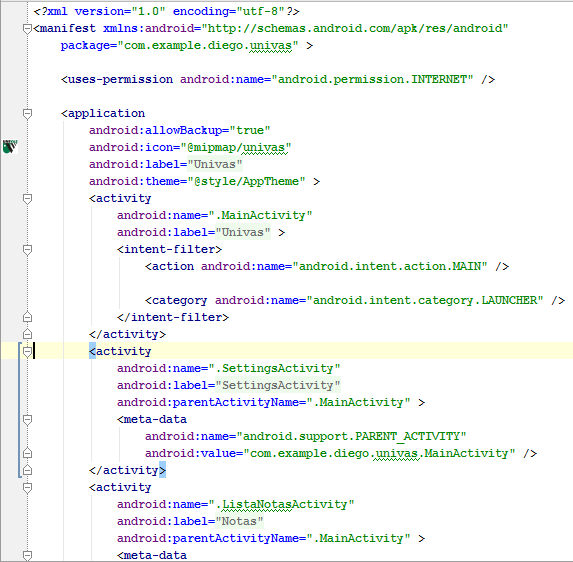
\includegraphics[scale=0.5]{./imagens/imagem10.png}}
			\caption[\texttt{AndroidManifest.xml}]{\texttt{AndroidManifest.xml}.
			 \textbf{Fonte:}Elaborado pelos autores.}
			\label{fig:exemplo10}
		\end{figure}

	\par O \textit{Android Studio} tem uma facilidade de se trabalhar com
controladores de versão, nesse caso foi escolhido o \textit{GitHub}. Nele foi
criado uma pasta e compartilhada entre os participantes e por fim configurou-se
o \texit{Git} com a IDE para que cada um possa ter a versão mais atualizada do
projeto.
	
	\pagebreak
	\par No que diz respeito à contrução do \textit{webservice}, foi necessário a
intalação e configuração de um ambiente de desenvolvimento compatível com as
necessidades apresentadas pelo \textit{software} e que foram levantadas através
dos requisitos. Foi instalado o \textit{Servlet Container Apache Tomcat} em sua
versão de número 7. O \textit{Servlet Container} foi instalado para que o
\textit{Web Service} pudesse fornecer os serviços necessários para o consumo de
dados do Aplicativo \textit{Android}, haja vista que \textit{Apache tomcat} faz
uso amplo do protocolo HTTP\footnote{HTTP - Hypertext Transfer Protocol} e da
plataforma \textit{Java} de desenvolvimento.
			
		\par Para armazenar os dados gerados e/ou recebidos foi necessário fazer a
	intalação do Sistema Gerenciador de Banco de Dados(SGBD) \textit{PostGreSql} na
	sua versão de número 9.2. Através de um levantamento de requisitos parciais e das
	reuniões entre os participantes foi possível construir um Diagrama de Entidade
	e Relacionamento, no qual ficou definido a estrutura do banco de dados da
	aplicação. A figura \ref{fig:exemplo5} mostra o Diagrama de Entidade e
	Relacionamento concebido para esta pesquisa.

		\begin{figure}[h!]
			\centerline{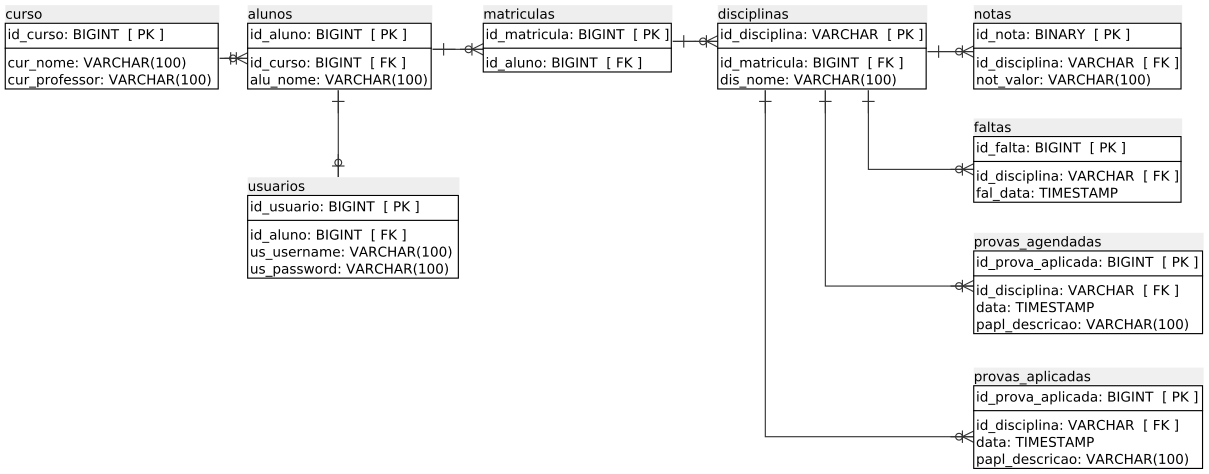
\includegraphics[scale=0.5]{./imagens/imagem5.png}}
			\caption[Diagrama de Entidade e Relacionamento]{Diagrama de Entidade e
			Relacionamento.
			\textbf{Fonte:}Elaborado pelos autores.}
			\label{fig:exemplo5}
		\end{figure}

		\par Fazendo uso desse diagrama foi possível criar todas as classes
	\textit{Java} que representam as entidades do mapeamento objeto-relacional. 
	Essas classes foram criadas fazendo uso de anotações próprias do
	\textit{Hibernate}, que é um \textit{framework} que implementa a especificação
	JPA\footnote{JPA - \textit{Java Persistense API}}. Essas classes fazem parte
	dos mecanismos de persistêcia de dados, e são simplesmente POJO's\footnote{POJO
	- \textit{Plain Old Java Object }} ou seja objetos simples que contêm somente
	atributos privados e os métodos \textit{getters} e \textit{setters} que servem
	apenas para encapsular estes atributos. Uma das classes criadas, foi a classe
	\texttt{Curso.java} que representa a tabela \texttt{cursos} no banco de dados e
	está representada no código \ref{fig:classecurso}.
	
	\pagebreak
	
	\begin{lstlisting} [style=custom_Java,caption={[Classe \texttt{Curso}]{Classe
	\texttt{Curso}. \textbf{Fonte:} Elaborado pelos autores.}},
	label=fig:classecurso] 
	@Entity(name = "cursos") 
	public class Curso {

			private Long idCurso;
			private String nome;
			private String professor;
		
			@Id
			@GeneratedValue
			@Column(name = "id_curso")
			public Long getIdCurso() {
				return idCurso;
			}
		
			public void setIdCurso(Long idCurso) {
				this.idCurso = idCurso;
			}
		
			@Column(length = 100, nullable = false)
			public String getNome() {
				return nome;
			}
		
			public void setNome(String nome) {
				this.nome = nome;
			}
		
			@Column(length = 100, nullable = false)
			public String getProfessor() {
				return professor;
			}
		
			public void setProfessor(String professor) {
				this.professor = professor;
			}
			
			/**
			 *hashCode e Equals
			 */
		}
	\end{lstlisting}
	
		\par Foram criadas outras classes \textit{Java} com a mesma finalidade da
	anterior, porém com pequenas diferenças no que diz respeito à atributos,
	metodos e anotações. Estas classes representam, de maneira individual, as
	tabelas no banco de dados. Certos atributos dessas classes tem por finalidade
	representar as colunas de cada tabela. Já os atributos que armazenam instâncias
	de outras classes ou até mesmo conjuntos(coleções) de intâncias representam os
	relacionamentos entre as tabelas. E por fim, para cada classe que representa um
	entidade, foi necessário implementar os métodos \texttt{hashCode} e
	\texttt{equals}, para que estas pudessem facilmente ser comparadas e
	diferenciadas em relação aos seus valores, haja vista que cada instância
	destas classes representa um registro no banco de dados.
		
		\par Em seguida à criação das entidades, foi necessário configurar o arquivo
	\texttt{persistence.xml} que fica dentro do \textit{classpath} do projeto
	\textit{Java} ou seja, dentro da mesma pasta onde estão contidos pacotes do
	projeto. Esse arquivo é extremamente importante pois, é nele que estão todas
	as configurações relativas à conexão com o banco de dados, configurações
	referentes ao Dialeto SQL que vai ser usado para as consultas e configurações
	referentes ao \textit{persistence unit} que é o conjunto de classes mapeadas
	para o banco de dados.	O arquivo \texttt{persistence.xml} está exposto no
	código \ref{fig:persistence}.
	
  \begin{lstlisting}[style=custom_XML,caption={[\texttt{persistence.xml}]
  {\texttt{persistence.xml}. \textbf{Fonte:} Elaborado pelos autores.}},
	label=fig:persistence]

		<?xml version="1.0" encoding="UTF-8"?>
		<persistence version="2.1"
			xmlns="http://xmlns.jcp.org/xml/ns/persistence" 
			xmlns:xsi="http://www.w3.org/2001/XMLSchema-instance"
			xsi:schemaLocation="http://xmlns.jcp.org/xml/ns/persistence
			http://xmlns.jcp.org/xml/ns/persistence/persistence_2_1.xsd">
				<persistence-unit name="WsUnivas">
					<provider>org.hibernate.ejb.HibernatePersistence</provider>
					<properties>
						<property name="javax.persistence.jdbc.url" value="jdbc:postgresql://localhost:5432/wsunivas" />
						<property name="javax.persistence.jdbc.user" value="postgres" />
						<property name="javax.persistence.jdbc.password" value="2289cpm22" />
						<property name="javax.persistence.jdbc.driver" value="org.postgresql.Driver" />
						<property name="hibernate.dialect" value="org.hibernate.dialect.PostgreSQLDialect" />
						<property name="hibernate.show_sql" value="true" />
						<property name="hibernate.format_sql" value="true" />
						<property name="hibernate.hbm2ddl.auto" value="update" />
					</properties>
				</persistence-unit>
		</persistence>
	\end{lstlisting}
		
			\par Em seguida à confecção do \texttt{persistence.xml} foi criada a
		classe \texttt{JpaUtil} que está representada na \ref{fig:classejpautil}.
		Esta classe é responsável por criar uma \texttt{EntityManagerFactory} que é
		uma  fabrica de instâncias de \texttt{EntityManager} que nada mais é que um
		\textit{persistence unit} ou unidade de persistência. Essa classe têm a
		responsabilidade de prover um modo de comunicação entre a aplicação e o banco
		de dados. Porém a classe \texttt{JpaUtil} cria uma única instancia de
		\texttt{EntityManagerFactory}, que é responsável por disponibilizar e
		gerenciar as instancias de \texttt{EntityManager} de acordo com a necessidade
		da aplicação.
		
		\pagebreak
		\begin{lstlisting} [style=custom_Java,caption={[Classe
		\texttt{JpaUtil}]{Classe \texttt{JpaUtil}. \textbf{Fonte:} Elaborado pelos autores.}},
	label=fig:classejpautil] 
		public class JpaUtil {
        private static EntityManagerFactory factory;

        static {
                factory = Persistence.createEntityManagerFactory("WsUnivas");
        }

        public static EntityManager getEntityManager() {
                return factory.createEntityManager();
        }

        public static void close() {
                factory.close();
        }

}
	\end{lstlisting} 



			\par Em seguida a construção das classes que fazem a parte da persistência de
		dados, foi desenvolvido a parte de disponibilização de serviços
		\textit{RESTful}, fazendo uso do \textit{framework} \textit{Jersey}. Foi
		necessário, portanto fazer a configuração da aplicação para que fazendo uso
		deste \textit framework a classe que representa o primeiro serviço do
		\textit{webservice}, que é a classe \texttt{Alunos}. Essa classe representa um contexto
		
		
